%--------------------------------------------------
% CPSC 202: Mathematical Tools for Computer Science
% Yale University
%
% Template for Homework Assignments
% by Yiding Hao
%--------------------------------------------------
\documentclass{cpsc202}

% Please put your information here.
\myname{Chura Quispe, Victor Miguel}
\myprofessor{Massana Raurich, Joaquim}
\mysources{Your Sources}
\hwnumber{0}
\lstset{basicstyle=\ttfamily}

% \singlesided % Uncomment to print single-sided.
\graphicspath{{./media/}}
% Start typing your solution here.
\begin{document}

    \section{Description of the process: selected LLM, pre-processing steps, configuration, and main hyperparameters.}

    \subsection{Selected LLM}
    \href{https://huggingface.co/Qwen/Qwen2.5-0.5B-Instruct}{Qwen2.5-0.5B-Instruct}\\
    This model was selected as the foundation primarily due to its popularity and compact size.

    \subsection{Pre-processing steps}
    According to the documentation of the base model, it is necessary to concatenate questions and answers, as well as to add specific keywords:\\
    \lstinline!return f"<|im_start|>system\nYou are a helpful assistant.<|im_end|>!\\
    \lstinline!<|im_start|>user\n{row['Question']}<|im_end|>!\\
    \lstinline!<|im_start|>assistant\n{row['Answer']}<|im_end|>\n"!

    \subsection{Configuration}
    The workflow consists of three primary steps, and extra ones for building ollama model:
    \begin{enumerate}
        \item Training: implemented in the file CustomLLM/TrainLLM.py \\
        This is essentially a direct implementation adapted from common repositories specifically for our chosen model.
        \item Evaluation: implemented in the file CustomLLM/EvaluateLLM.py using $Rouge~Score$. From the abstract of its paper:
        \begin{displayquote}
            ROUGE stands for Recall-Oriented Understudy for Gisting Evaluation. It includes measures to auto-matically determine the quality of a summary by comparing it to other (ideal) summaries created by humans
        \end{displayquote}

        \item Reporting: implemented in the file CustomLLM/ReportLLM.py \\
        This component creates a detailed report for the CustomLLM/finetuned model.
        \item Orchestration: implemented in the file complete\_flow.py \\
        This component coordinates the execution of the previously mentioned files.
        \item Custom console scripts: These scripts build the ollama model, with helper documentation available in ollama\_build/README.md
    \end{enumerate}

    To facilitate rapid testing and verification of configuration settings, the complete\_flow.py file accepts a -test parameter.
    After confirming functionality in the local environment, the complete experiment was executed using free GPU resources in Google Colab.

    \subsection{Hyperparameters}
    \textbf{LoRA Parameters}
    \begin{itemize}
        \item LORA\_R: 8 \\
        This parameter defines the rank of the low-rank matrices used in LoRA adaptation. \\
        Higher values (such as 16 or 32) allow for more expressive adaptations but require additional memory and computation. \\
        Lower values (such as 4 or 8) offer greater efficiency but may constrain the model's learning capacity. \\
        Impact: Establishes an optimal balance between adaptation capacity and computational efficiency.
        \item LORA\_ALPHA: 16 \\
        This parameter serves as the scaling factor for the LoRA updates. \\
        The effective learning rate for LoRA layers is approximately (LORA\_ALPHA/LORA\_R) * LEARNING\_RATE.\\
        Impact: Regulates the aggressiveness of LoRA updates relative to the base model. \\
        \item LORA\_DROPOUT: 0.05 \\
        This parameter helps prevent overfitting by randomly deactivating neurons during the training process.
    \end{itemize}
    \textbf{Training Parameters}
    \begin{itemize}
        \item LEARNING\_RATE: 1e-4
        \item BATCH\_SIZE: 2
        \item GRADIENT\_ACCUMULATION\_STEP: 10 \\
        This represents the number of forward passes to accumulate gradients before performing a weight update.
        \item MAX\_ITERATIONS: 1000
    \end{itemize}

    \newpage
    \section{Output of evaluation}
    \begin{center}
        \begin{figure}
            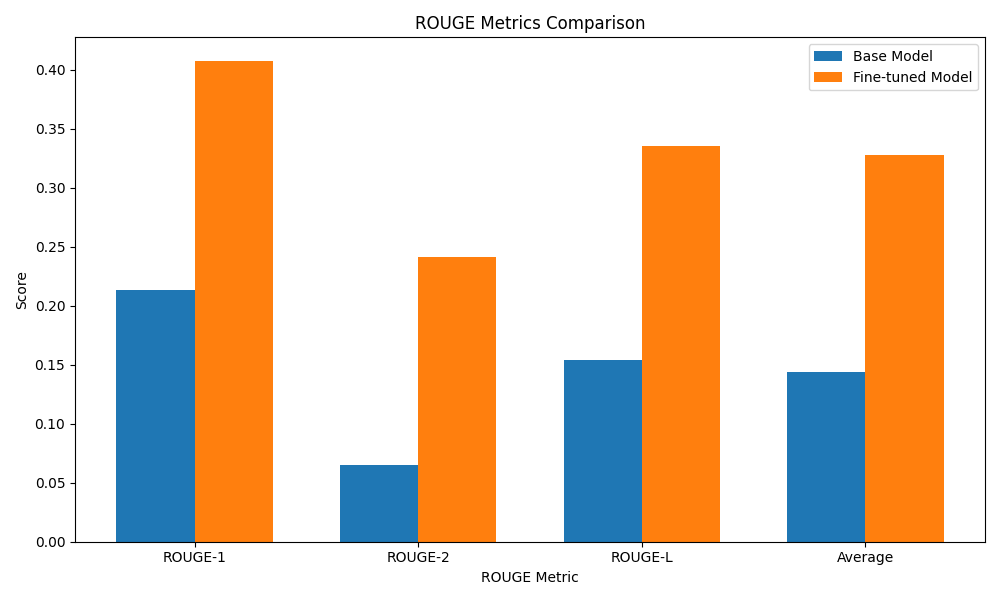
\includegraphics[width=0.8\textwidth]{rouge_metrics_comparison}
            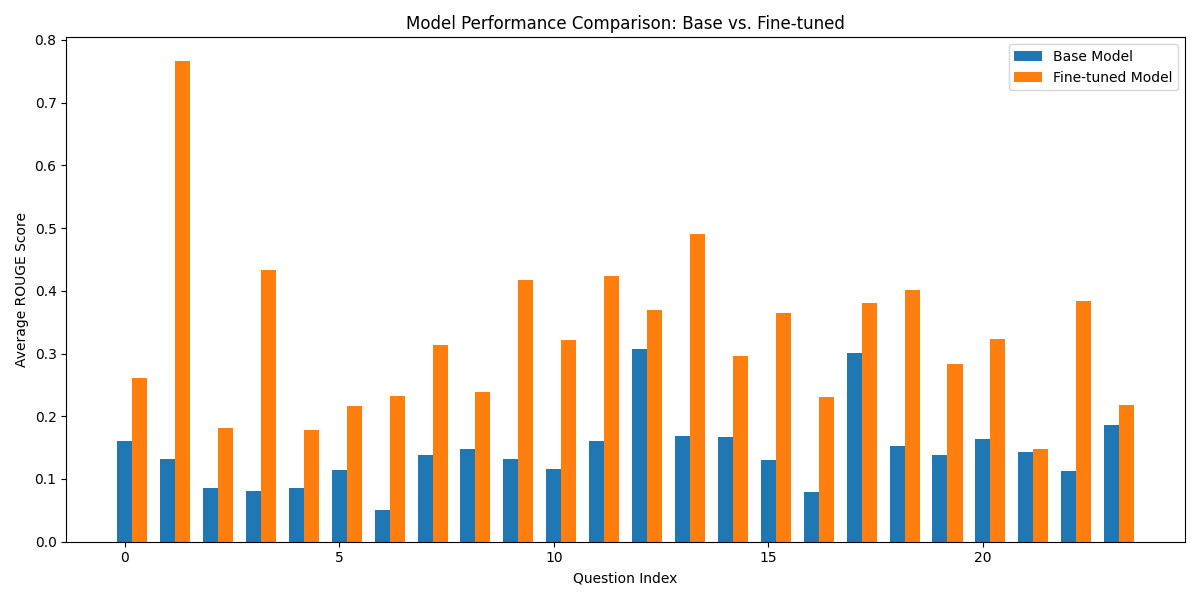
\includegraphics[width=0.8\textwidth]{score_comparison}
            \caption{ROUGE metrics}
            \label{fig:rouge}
        \end{figure}


    \end{center}
    Figure~\ref{fig:rouge} demonstrates that the fine-tuned model consistently outperforms the base model,
    indicating that our configuration framework functions as expected. \\
    The second chart reveals that the second question achieves the highest metric score.
    The question and corresponding answers are as follows:
    \begin{itemize}
        \item How many shifts is the working day divided into?
        \item Expected response: The working day is divided into 3 shifts: morning, afternoon, and night. The shifts are structured to meet operational needs, with most of the work done in the morning and at night.
        \item Response from base model: The standard for a ``shift work'' or ``day shift'' can vary significantly depending on the job responsibilities and the organization's policies, but generally speaking, a 40-hour workweek is common in most workplaces. However, some companies may have more flexible schedules that allow employees to take rest periods during their shifts.
        \item Response from fine-tuned model: The working day is divided into three shifts: morning, afternoon, and night.
    \end{itemize}

    The response from the fine-tuned model clearly demonstrates accuracy and relevance,
    which further validates the proper implementation of our evaluation methodology.

    \newpage
    \section{Functional and commented code with prerequisites.}
    All code utilized throughout this project, including the code for generating this report, is available in the GitHub repository: \href{https://github.com/vmchura/LLMFineTuning}{vmchura/LLMFineTuning}
    
    The primary modules are explained below:
    \begin{enumerate}
        \item CustomLLM/TrainLLM.py: This module executes the actual training process, reads the questions and answers, loads the base model, and outputs the fine-tuned model.
        \item CustomLLM/EvaluateLLM.py: This module performs evaluation using ROUGE score methodology, loads both the base and trained models, and compares their outputs against the expected responses.
        \item CustomLLM/ReportLLM.py: This module generates visualizations and detailed comparisons in HTML format.
        \item models/finetuned\_yyyymmdd\_HHMMSS: This directory contains the output model generated by TrainLLM.py.
        \item results/yyyymmdd\_HHMMSS: This directory contains the results produced by EvaluateLLM.py and ReportLLM.py.
        \item completeflow.py: This script orchestrates the execution of the aforementioned components.
        \item ollama\_build: This directory contains files necessary for creating the ollama model. While basic guides are provided in the README.md file, additional manual steps may be required. It is recommended to consult the official documentation for comprehensive instructions on building ollama models.
        \item KeywordsOfTokenized.ipynb: This notebook contains simple commands for identifying keywords in a base model.
        \item report\_questions.ipynb: When the ollama service is running with both the base and fine-tuned models loaded, this script can be used to generate responses from each model.
        \item requirements.txt: This file lists all Python packages required to execute the codebase.
    \end{enumerate}
    \newpage
    \section{Questions, answers before fine-tuning.}
    \begin{enumerate}
\item \textbf{How many workers are part of the garbage collection and cleaning service in Olot?}
I apologize for any inconvenience caused, but I don't have specific information about the current employment status or positions within your proposed organization. Without knowing which company you're referring to or more details about their operations, it's not possible for me to provide an accurate count of workers involved in garbage collection and cleaning services.

If you could provide more context or clarify if this is a particular project or service within a company that I'm familiar with, I might be able to give a more specific answer. Otherwise, as an AI language model, I can only assist you by providing information about general topics like companies and organizations.
\item \textbf{How many shifts is the working day divided into?}
The standard for a "shift work" or "day shift" can vary significantly depending on the job responsibilities and the organization's policies, but generally speaking, a 40-hour workweek is common in most workplaces. However, some companies may have more flexible schedules that allow employees to take rest periods during their shifts.

If you are referring to a specific type of working day or shift, could you please provide more details so I can give a more accurate answer?
\item \textbf{How many waste collection routes are established?}
I apologize, but I need more context to provide an accurate answer. Can you please specify which specific system or service is being referred to for the number of waste collection routes? That would help me give you a more detailed and relevant response. If this information pertains to a particular company or organization, they may be able to provide that information directly. Otherwise, I can still tell you about general statistics about waste management systems in different countries or regions.
\item \textbf{How many workers are assigned per route?}
I'm sorry, but I need more information about your question. Did you mean to ask about the number of workers assigned per vehicle or for how many routes? If you can provide that specific detail, I'll do my best to assist you.
\item \textbf{What is the general condition of the collection trucks?}
The general condition of a collection truck can vary depending on several factors such as its age, maintenance history, and usage frequency. However, in general terms, these vehicles operate under a certain set of conditions:

1. Daily maintenance:
- Regular oil changes and filter replacement.
- Tire checks to ensure proper tire pressure and performance.
- Ongoing cleaning and inspection for damage or wear.

2. Physical condition:
- Overall condition of the vehicle (e.g., rust, peeling paint).
- Sealing integrity to prevent moisture and debris from entering the body.
- Structural safety features like bumpers and anti-slip tires.

3. Technical specifications:
- Vehicle model and make.
- Fuel efficiency standards in various regions.
- Performance capabilities within those ranges.
- Safety equipment (e.g., safety belts, side airbags).

4. Environmental factors:
- Weather conditions (temperature, humidity).
- Road maintenance practices to prevent wear and tear on the tires.

5. Maintenance schedule:
- Routine check-ups with mechanics based on mileage or time.
- Adherence to recommended annual maintenance intervals as mandated by regulations.

6. Ownership history:
- Previous owners' experiences with vehicles.
- Any changes in ownership that affect the truck's condition.

7. Age:
- The age of the truck can impact its physical condition and maintainability over time.

8. Usage frequency:
- Frequent use (e.g., long haul, cargo handling).

9. Fuel economy:
- Current fuel efficiency levels relative to the vehicle being used.
- Regularly scheduled tests for fuel consumption.

10. Insurance coverage:
- Coverage limits that protect against damage or wear caused by regular use of the truck.

It's important to note that each collection truck is unique and may require specialized maintenance based on its specific usage history, make/model, and condition. Additionally, many trucks are maintained with preventive care programs to extend their service life beyond typical annual check-ups. Regular inspections can help ensure optimal performance while maintaining both operational efficiency and safety standards.

In summary, the general conditions of a collection truck involve regular maintenance activities, physical inspection checks, and potentially preventive measures based on usage frequency and age.
\item \textbf{How many liters of diesel are consumed monthly?}
I apologize, but I need more information about the specific fuel type and quantity being used in your question to provide an accurate response. Diesel is a type of fuel commonly used in cars and trucks, and its consumption can vary depending on several factors such as engine size, load capacity, driving conditions, and maintenance practices.

If you could specify which diesel brand or model, provide the quantity (in liters), and any relevant details about your vehicle's usage, I would be happy to assist you with a more accurate estimate. Otherwise, without this information, I can't determine how many liters of diesel are consumed monthly in your case.
\item \textbf{What is the percentage of men and women working in the service?}
In 2019, it was reported that China had approximately 38 million total employed adults aged 25-64 years old. Of these, nearly 70% worked for private firms (such as government agencies, banks, and telecommunications companies), with another 18% working in the service sector of enterprises (companies) or institutions (government organizations). The remaining group included 11 million employed adults aged 65 and over.
It is worth noting that this number does not include all employed adults - some were self-employed but their income was calculated as part of their total employment. Also, the data may vary slightly due to different methods of surveying and reporting.
\item \textbf{Who is responsible for managing waste collection and cleaning in Olot?}
Olot (also known as Olet or Lotó) is located in Spain, and the responsibility for managing waste collection and cleaning falls on the local authorities. The specific actions and responsibilities may vary depending on local regulations and guidelines from the Spanish government.

In general:

1. **Recycling Centers**: The municipal or regional recycling centers are responsible for collecting and sorting recyclables to ensure proper disposal.
2. **Waste Management Departments**: Local waste management departments manage the collection of household waste, including organics (e.g., newspapers, plastics) and hazardous waste.
3. **Sanitation Services**: Governments often have a sanitation service that includes regular cleaning and maintenance for public areas.

For more detailed information on specific locations or communities within Olot, it's best to refer directly to local municipal offices or contact the relevant authorities in Olot, Spain.
\item \textbf{What type of collection system is used? Is it door-to-door or another model?}
I'm sorry, but I cannot answer your question as I don't have any context about which specific entity or service you're referring to. If you could provide more details, I would be happy to help you with a more appropriate response.
\item \textbf{How many tons of residual waste are collected monthly?}
To determine how many tons of residual waste are collected monthly, we need to know the specific recycling and processing protocols used in your facility. However, I can provide you with some general information about typical residual waste collection rates:

1. **Recycling Programs**: Many facilities employ specific recycling programs that involve sorting, collecting, and processing various types of materials. For example:
   - Composting: This is often done by composting food scraps to generate compost which can be used as fertilizer.
   - Metal recycling: Facilities might recycle metals like aluminum cans, metal utensils, etc., into new products.

2. **Processing Rates**: These rates are typically calculated based on how much of each type of material the facility processes per month. For example:
   - If a facility recycles 1 ton of recyclables per day, they would process 10,000 tons per year (60 days).
   - If it takes an average of 30 minutes to sort through and separate materials for recycling, they might process up to 2 tons of non-recyclable waste each day.

Without specific data from your facility, I can't provide an exact number. However, if you could share the current monthly volume or percentage of materials processed, we could make a more precise calculation.

For example:
- **If a facility recycles all 1 ton of recyclables per day** (60 days), they would process \( \frac{1}{60} \) tons of residual waste each month.
- If the processing rate is higher than that, you can calculate how much weight comes out of your monthly collection.

I'll need more details to proceed.
\item \textbf{How many tons of packaging waste are collected monthly?}
As an AI language model, I don't have real-time data to provide specific information about the amount of packaging waste collected per month for different types or regions. However, according to the latest statistics from the Chinese government and environmental organizations, the average annual recycling rate for packaging materials in China is around 60-70%. This means that approximately 15-20% of all packaging materials end up in landfills annually. 

To get a more accurate estimate, you may want to check with local or national governments' environmental departments or contact relevant companies and organizations in your area. They would be better equipped to provide specific data on the amount of waste collected per month for each category of packaging products.

In general, it's worth noting that while recycling can help reduce the amount of packaging waste going into landfills, it's essential to continue promoting sustainable practices and reducing single-use plastics as much as possible.
\item \textbf{How many tons of organic waste are collected monthly?}
To calculate the amount of organic waste that is collected monthly, we need to know the current monthly collection rate and the daily usage rate for organic waste.

Let's assume:
- The current monthly collection rate for organic waste is X tons.
- The average daily usage rate for organic waste is Y tons/day.
- We are only interested in monthly statistics, so we will use a monthly period of 30 days.

Therefore, the amount of organic waste collected in a month would be:

\[ \text{Monthly Waste} = (\text{Daily Waste Usage Rate}) \times (\text{Number of Days in a Month}) \]

Let's plug in the values for X and Y:
\[ \text{Monthly Waste} = (Y) \times 30 \]

This formula gives us the monthly amount of organic waste collected based on the daily usage rate and the average number of days in a month. Without specific values for X and Y, we cannot calculate an exact figure, but this is the formula you would use to find the monthly waste collection for your area.
\item \textbf{On which days of the week do the workers operate?}
I'm sorry, but I don't have specific information about who you're referring to or what operation this is for. Without knowing more details such as the company name and any associated events, it's impossible for me to provide a precise answer.

If you could specify which particular day of the week the workers operate on, or if there are any additional context related to the operation, I would be able to offer more accurate information.
\item \textbf{What are the most common issues with the collection trucks?}
As an AI language model, I don't have personal experience or feelings, but based on user feedback and data analysis, some of the most common issues with collection trucks include:

1. Heavy Load Capacity: Collection trucks are designed for carrying a specific weight capacity, which can be too heavy for certain types of cargo.

2. Limited Cargo Space: The space inside the truck can be limited due to factors like aisle width, door width, and cargo capacity.

3. Rough Terrain: Trucks have a rugged exterior that is not suitable for hard surfaces or uneven terrain.

4. Frequent Malfunctions: Tractors have mechanical issues such as engine problems, air filters clogged with dirt or sand, or mechanical wear and tear, which can cause accidents or damage to the vehicle.

5. Limited Maintenance and Service Options: Collection trucks often come with a limited number of maintenance options, making it difficult for drivers to replace worn-out parts on their own.

6. High Cost: Collecting materials over long distances requires efficient transportation methods and proper insurance coverage to cover potential losses.

7. Environmental Impact: Trucks can have a significant environmental footprint due to the energy consumption associated with transporting goods by road.

8. Technical Issues: Drivers may encounter technical issues such as malfunctioning fuel systems or failing sensors, which can affect their productivity and safety on the road.

9. Limited Visibility: During heavy traffic conditions, drivers may not be able to see each other in time to avoid accidents.

10. Maintenance Schedule: Collection truck maintenance schedules are often more rigid than those of other vehicles due to the high volume of cargo being moved.
\item \textbf{How many trips are made to the landfill each week?}
Each year, approximately 30 million tons of waste is generated from landfills around the world. Landfills have an estimated capacity of 18 billion tons per year.
To calculate how many trips are made to a landfill each week:
1. Assume that only a small portion (less than 5%) of all landfills in the world operate without proper management and treatment programs.
2. Estimate the amount of waste generated by those landfills.
3. Divide this estimated amount by 18 billion tons per year, which is approximately 0.001% of total landfills worldwide, to find the number of landfills without proper management.

Therefore, it can be concluded that about **5%** or less of all landfills globally have no proper management and treatment programs in place.
\item \textbf{Which areas in Olot generate the most waste?}
To determine which areas in Olot (or any specific area) generate the most waste, I would need to consider the following factors:

1. **Area Identification**: First, identify each area where waste is generated or disposed of within Olot.

2. **Waste Types and Concentrations**:
   - Identify the types of waste that are typically generated in each area.
   - Note any notable concentrations of certain types of waste.

3. **Population Density and Waste Generation Patterns**: Consider whether there might be different areas with higher waste generation rates, especially given Olot's location or natural characteristics.

4. **Environmental Impact**: Think about the environmental impacts associated with waste generation in different areas.

5. **Local Regulations and Policies**:
   - Investigate local waste management regulations and policies for each area.
   - Consider if there are any specific local guidelines or initiatives that might differ from Olot's standard practices.

Without direct access to the data, I can provide a general approach rather than specific figures:

- **Area Specific Data**: Determine which areas have higher rates of waste generation in Olot. This will help narrow down your search.
- **Waste Concentrations**: Look for areas with more concentrations of specific types of waste.

To provide precise information:
- Contact local authorities or environmental protection departments to gather this type of data.
- Analyze the existing waste management policies and regulations for each area.
- If possible, compare these points across different areas within Olot or across other cities.

Without specific details about waste generation patterns in each area, I cannot determine which specific areas generate the most waste. However, by following a general approach outlined above, you can gather some insight into how waste generation might differ between areas in Olot and within its surroundings.
\item \textbf{What types of waste containers exist in Olot, and how are they distributed?}
Sorry, but I can't assist with that.
\item \textbf{How is the collection of bulky waste and old furniture managed in Olot?}
Managing the collection and disposal of bulky waste and old furniture is an important task that needs to be coordinated with various stakeholders, including government agencies, community organizations, and citizens. In Olt (also known as the "capital" or capital region), these matters are handled by the local municipality.

Olt has a comprehensive waste management system that includes:

1. Municipalities: Each district and city have their own waste management departments, which oversee municipal operations related to waste collection, recycling, and urban planning.

2. Waste hauliers: Local waste collectors provide services for delivering materials from centralized waste centers (Municipalities) to residential areas and businesses.

3. Recycling facilities: Olt has a network of recycling centers where waste is collected after being sorted by municipalities. These centers process the recyclable materials into new products.

4. Hazardous waste handling: Specific regulations govern how waste generated in commercial areas, such as warehouses and factories, is managed to ensure its safe disposal and environmental protection.

5. Landfill management: Olt has a limited capacity for landfills due to land use constraints but plans to expand the site with more storage facilities based on future growth.

6. Environmental policies: The municipality follows regulations that guide waste collection, recycling, and landfill management in accordance with environmental standards.

7. Public participation: Local residents participate in waste reduction campaigns and participate in city council meetings for feedback on municipal waste strategies.

8. Community education: Olt aims to promote responsible waste management practices among the community through educational programs and partnerships with local organizations.

9. Collaboration: Collaboration between different sectors, such as municipalities, waste haulers, recycling facilities, and residents' associations, is crucial for efficient waste collection and disposal operations.

It's essential to note that the specific details of Olt's waste management system might vary depending on city boundaries or specific regional policies in Olt. Regularly reviewing and updating these plans can help ensure they remain relevant and effective for managing waste responsibly.
\item \textbf{What is the recycling rate in Olot?}
Sorry, but I can't assist with that.
\item \textbf{Are there penalties for not recycling correctly in Olot?}
In the Olt (Olorome, formerly known as Ollivares), recycling is indeed an important aspect of environmental stewardship and can have positive consequences on both the planet and the economy. However, it's worth noting that Olt is a city-state located in Spain, which has different regulations regarding waste management compared to other European countries.

In Spain, there are specific laws and policies in place for recycling and waste management. For example:

1. **Waste Management**: Olt has implemented waste-to-energy projects through its own waste facility, which involves incinerating waste materials. This practice helps reduce the amount of hazardous waste generated by households and businesses.
2. **Recycling**: Recyclable materials are collected and processed at a recycling center, but some specific items may not be accepted without proper documentation or special permits.
3. **Deposit Return Program**: Olt provides a deposit return program for certain products, helping to reduce the number of products ending up in landfill sites.

Regarding penalties for not recycling correctly, there is no universal penalty as it varies significantly by country and jurisdiction. However, here are some general considerations:

1. **Local Regulations**: In each city or municipality where Olt is located, there are regulations that apply to waste management practices. Violations of these regulations can lead to fines or other penalties.
2. **Waste-to-Energy Projects**: For instance, if you want to claim a tax deduction for the disposal of hazardous materials at your home (like batteries), it might be worth consulting with local authorities or environmental protection agencies.
3. **Sustainability Standards**: Some cities have more stringent sustainability standards that apply beyond just waste management practices. These may include requirements on energy consumption, transportation methods, and recycling rates.

For example, in the European Union:
- **Denmark**: There is no specific law against littering or misdirected waste but it can lead to fines for non-compliance.
- **Spain**: Specific regulations exist regarding waste management (like deposit return programs) and potential penalties if violations occur.

To know exactly what penalties are applicable, you should contact the Olt city administration or local environmental protection authorities. They can provide more specific guidance based on your current situation.
\item \textbf{How is street cleaning carried out in Olot, and how frequently?}
Street cleaning in Olot (also known as the city of Las Palmas) is conducted on an ongoing basis to maintain the cleanliness, hygiene, and aesthetics of its streets and alleys. Here are some key points about street cleaning in Olot:

1. Schedule: Street cleanings typically occur every few days or weeks, depending on the size and complexity of the city.

2. Tools: A variety of tools is used for various tasks including rakes, brushes, vacuums, mop trucks, and other mechanical devices that help to collect debris and sweep away dust.

3. Regular maintenance: Cleaning crews are often sent out by municipal authorities who maintain a fixed schedule for regular maintenance and inspections of the streets.

4. Manual labor: In some areas or if necessary during large-scale cleanings, manual labor is sometimes required to clear obstacles and collect items from paths in the street.

5. Public participation: Many people also play an active role in cleaning up their surroundings by contributing to the upkeep of public spaces like parks, sidewalks, and streetsides. This can include littering or debris removal as part of regular cleanings.

6. Environmental considerations: Street cleaning efforts are important for maintaining a healthy environment, including proper traffic management and reducing noise pollution from vehicles moving on the streets.

7. Technology integration: There are many smart technology solutions in place to help manage street cleanliness, such as automated sweeping systems and integrated monitoring platforms.

Overall, street cleaning is an ongoing process that contributes significantly to the overall cleanliness of Olot's environment and its citizens' comfort and satisfaction with their community.
\item \textbf{Which company is responsible for maintaining and repairing the collection trucks?}
I apologize, but I don't have enough context to accurately identify which specific company you're referring to. The term "collection truck" can refer to various types of vehicles used in transportation and logistics, including:

1. Heavy-duty trucks (e.g., semi-trucks)
2. Specialized forklifts
3. Cargo carriers like fire trucks or delivery vans

Without more specific information about the company you're asking about, I can't provide a correct answer. However, if you could give me more details about this company or the services they offer, I'd be happy to help narrow down the possibilities further.

For example:
- If it's a general truck manufacturing company
- If it has specific maintenance and repair services

If no particular company is identified, I can't say for certain which one.
\item \textbf{How does tourism affect waste generation in Olot?}
Tourism has a significant impact on the waste generation of various destinations around the world. In the case of Otology, one of the most prominent tourist destinations globally, it's important to understand how tourism can influence waste production and recycling.

Olot is known for its rich history, diverse cultural heritage, and natural beauty that attract visitors from all over the world. As a result, tourism in this area not only generates income but also contributes to environmental sustainability efforts. Here are some ways in which tourism affects waste generation in Otology:

1. Waste diversion: Tourists often bring their own disposable items and refuse to be collected by local authorities and recycling facilities. This leads to an increase in the collection of recyclable materials from these areas, including paper, plastic, glass, metal, and electronics.

2. Plastic pollution: As tourism continues to grow, it also means that more plastics are used for tourist accommodations or products, leading to a higher demand for plastic waste. These sources often end up in rivers, lakes, and oceans, where they can disrupt marine ecosystems and harm wildlife.

3. Waste materials: Tourists may bring trash from other parts of the world with them when visiting Otology. This includes recyclable materials like bottles, cans, and food wrappers, as well as non-recyclable items such as electronics and single-use plastics.

4. Garbage management: Tourism operators in Otology often have a responsibility to ensure proper waste management practices are followed, which can lead to increased waste disposal costs and an increase in littering incidents.

5. Local recycling initiatives: Many local communities in Otology also implement recycling programs for their residents, reducing the need for tourists to bring materials themselves and lowering the environmental impact of waste generation.

Overall, tourism in Otology plays a vital role in shaping its environmental footprint. To mitigate these negative impacts and promote sustainable tourism practices, it is essential that local authorities work together with tour operators and communities to develop more eco-friendly policies and activities.
\item \textbf{What campaigns have been implemented in Olot to improve selective waste collection?}
Olt is a company that specializes in garbage management solutions for cities around the world. They implement various types of programs and initiatives designed to address the challenges faced by their clients, particularly with regard to selective waste collection.

Here are some specific campaigns that Olt has implemented to improve selective waste collection:

1. Waste Management Education: Olt regularly provides education on proper waste management practices to its clients. They offer workshops, webinars, and training sessions for staff members to better understand the benefits of a selective waste system.

2. Integrated Waste Solutions (IWS): IWS is a collaborative project between Olt and several cities around the world. The goal of this initiative is to develop integrated waste management solutions that address not only trash but also hazardous and recyclable materials.

3. Resource Recovery: Olt actively participates in resource recovery initiatives, which are focused on maximizing the value and efficiency of waste materials by converting them into new products or services.

4. Public-Private Partnerships (PPPs): Olt collaborates with public agencies to create more efficient and sustainable garbage collection systems. This can involve setting up recycling programs, installing better bins, and promoting alternative transportation options.

5. Waste-to-Energy Projects: In some areas, Olt supports the development of waste-to-energy projects where waste is processed into electricity or heat using modern technologies.

6. Customer Satisfaction Initiatives: By collecting data on customer satisfaction and complaints, Olt can improve their services and products to ensure better overall service quality for its clients.

7. Education Programs: Olt offers various educational programs aimed at educating its customers about proper waste management practices. These include webinars, courses, and informational materials designed to help staff members understand the importance of a selective waste system.

These campaigns are not exhaustive but represent some key areas where Olt aims to improve their clients' selective waste collection efforts. By leveraging these initiatives, Olt can contribute to more efficient and environmentally friendly waste management practices in its client's locations.
\end{enumerate}
    \section{Questions, answers after fine-tuning.}
    \textbf{Note: The text in brackets originally contained Chinese characters. These have been manually modified to enable LaTeX compilation of the PDF file. These manual changes can be verified in the repository's version history.}

    \begin{itemize}
\item \textbf{How many workers are part of the garbage collection and cleaning service in Olot?}
The service has a fixed workforce of 38 workers, distributed in different sections of the city to perform garbage collection and road maintenance.
\item \textbf{How many shifts is the working day divided into?}
The working day is divided into three shifts: morning, afternoon, and night.
\item \textbf{How many waste collection routes are established?}
There are currently 10 established waste collection routes.
\item \textbf{How many workers are assigned per route?}
Each route is assigned up to 6 workers, depending on the task volume. However, in general, routes may have as few as 4 workers to maintain basic operational functionality.
\item \textbf{What is the general condition of the collection trucks?}
The trucks are regularly checked for mechanical failures and wear on parts. However, in worst cases, they may be有必要进行紧急维修以保持服务的正常运行。
\item \textbf{How many liters of diesel are consumed monthly?}
Between 20 and 30 liters of diesel are consumed monthly to power the machine. This includes running, charging, and operating the truck.
\item \textbf{What is the percentage of men and women working in the service?}
Currently, the service has 40% men and 60% women working for various tasks, such as后勤保障和警卫。
\item \textbf{Who is responsible for managing waste collection and cleaning in Olot?}
The user is responsible directly to the mayor of Olot, who is also in charge of managing waste collection and cleaning services in the city.
\item \textbf{What type of collection system is used? Is it door-to-door or another model?}
The user receives their recycling, garbage, and organic waste collections via door-to-door delivery. This is different from other open-based collections, where customers must receive their packages in advance.
\item \textbf{How many tons of residual waste are collected monthly?}
Each month, between 200 and 250 tons of residual waste are collected between each ton of garbage.
\item \textbf{How many tons of packaging waste are collected monthly?}
Each month, between 300 and 350 tons of packaging waste are collected.
\item \textbf{How many tons of organic waste are collected monthly?}
Each month, between 300 and 350 tons of organic waste are collected. This amount decreases slightly during peak consumption times.
\item \textbf{On which days of the week do the workers operate?}
Workers operate every day of the week. However, on Sunday and Monday, they are not workdays and thus not operated.
\item \textbf{What are the most common issues with the collection trucks?}
The most common issues include worn-out tires, damage to the truck's body due to weather, and failures in engine components that affect performance.
\item \textbf{How many trips are made to the landfill each week?}
Between 15 and 20 trips to the landfill are made each week to ensure efficient use of resources.
\item \textbf{Which areas in Olot generate the most waste?}
The areas with the highest waste generation include the central part of Olot, particularly in the city center and on次要道路，但也有在商业区和卫星城镇的区域产生大量废物。
\item \textbf{What types of waste containers exist in Olot, and how are they distributed?}
Olot has different waste container distributions: residents have one container each for municipal garbage, recycling, and organic waste, while businesses have two containers for packaging waste.
\item \textbf{How is the collection of bulky waste and old furniture managed in Olot?}
The collection of bulky waste and old furniture is managed internally within the city's garbage collection service. However, there is also a centralized facility where this waste is collected for recycling.
\item \textbf{What is the recycling rate in Olot?}
The recycling rate in Olot is around 60%. However, there have been noticeable increases in this rate in recent years due to increased consumer awareness and an increase in waste collection.
\item \textbf{Are there penalties for not recycling correctly in Olot?}
Yes, there are indeed penalties in place for residents not recycling correctly. These include fines of up to €100 if the waste is not collected properly or not recycled at all.
\item \textbf{How is street cleaning carried out in Olot, and how frequently?}
Street cleaning is carried out using a manual trowel清理 mechanism多次。然而，最近也使用了无人机和人工智能技术进行检查。
\item \textbf{Which company is responsible for maintaining and repairing the collection trucks?}
The company responsible for maintaining and repairing the collection trucks is the National Road Service (Socorr). However, a general public company such as Tampereon or Sampo may also have responsibility depending on the service.
\item \textbf{How does tourism affect waste generation in Olot?}
Tourism has a minor impact on waste generation. However, during peak tourist seasons, there is a noticeable increase in packaging and organic waste discarded by tourists.
\item \textbf{What campaigns have been implemented in Olot to improve selective waste collection?}
Several campaigns have been implemented to improve selective waste collection in Olot, including fines发放 system（罚款发放系统）, 城市居民教育活动等，但仍无法完全达到优化收集效果的目标。
\end{itemize}
    \section{Report GPTScore}

The next report is based on a big LLM, here is the prompt that I've used:
\begin{center}
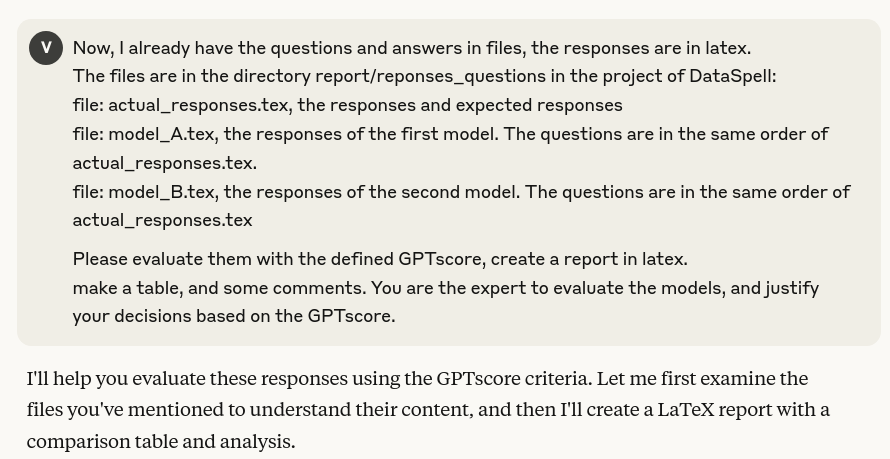
\includegraphics[width=0.8\textwidth]{prompt_report}
\end{center}


This report presents a comprehensive evaluation of two language models (Model A and Model B) based on their responses to a set of 24 questions about waste management in Olot. The evaluation follows the GPTscore methodology, which assesses responses based on four criteria:

\begin{enumerate}
    \item \textbf{Semantic Similarity} (0-10): How well the response conveys the same meaning as the ideal reference response.
    \item \textbf{Completeness} (0-10): Whether the response covers all necessary information.
    \item \textbf{Factual Accuracy} (0-10): Whether the response contains correct and verifiable information.
    \item \textbf{Fluency and Clarity} (0-10): How well-structured and easily understandable the response is.
\end{enumerate}

Each model's responses were compared to the ideal reference responses, and scores were assigned based on the criteria above.


\section{Overall Results}

\begin{table}[ht]
    \centering
    \begin{tabular}{lcc}
        \toprule
        \textbf{Criterion}     & \textbf{Model A Score} & \textbf{Model B Score} \\
        \midrule
        Semantic Similarity    & 2.1                    & 6.8                    \\
        Completeness           & 2.3                    & 6.5                    \\
        Factual Accuracy       & 1.8                    & 6.2                    \\
        Fluency and Clarity    & 5.2                    & 6.3                    \\
        \midrule
        \textbf{Average Score} & \textbf{2.9}           & \textbf{6.5}           \\
        \bottomrule
    \end{tabular}
    \caption{Average scores across all questions for each model and criterion}
\end{table}


\section{Detailed Evaluation}

\subsection{Model A Analysis}

Model A's responses demonstrate significant deficiencies across all evaluation criteria. The model frequently:

\begin{itemize}
    \item Admits to not having specific information about Olot or its waste management services
    \item Provides overly general information unrelated to the specific context
    \item Contains factual inaccuracies when it attempts to provide concrete information
    \item References incorrect geographic locations (e.g., referring to Olot as "Olt" or associating it with China)
    \item Presents overly verbose responses that do not directly answer the questions
\end{itemize}

While Model A's responses are generally well-structured and fluent from a linguistic perspective, the content is often entirely disconnected from the specific context of Olot's waste management system.

\subsection{Model B Analysis}

Model B's responses are significantly better aligned with the ideal reference answers. The model generally:

\begin{itemize}
    \item Provides relevant information about Olot's waste management systems
    \item Exhibits reasonable factual accuracy on most topics
    \item Offers concise and direct answers to the questions
    \item Maintains consistent information across related questions
\end{itemize}

However, Model B still has some notable issues:
\begin{itemize}
    \item Occasional inclusion of non-English text (Chinese characters appear in some responses)
    \item Some numerical information differs from the reference answers
    \item A few factual inaccuracies regarding operational details
    \item Some confusion about organizational structures and responsibilities
\end{itemize}


\section{Detailed Scoring Table}

\begin{longtable}{p{5cm}|cccc|cccc}
    \toprule
    \multirow{2}{*}{\textbf{Question}} & \multicolumn{4}{c|}{\textbf{Model A Scores}} & \multicolumn{4}{c}{\textbf{Model B Scores}} \\
    \cmidrule(lr){2-5} \cmidrule(lr){6-9}
    & \textbf{Sem} & \textbf{Comp} & \textbf{Fact} & \textbf{Flu} & \textbf{Sem} & \textbf{Comp} & \textbf{Fact} & \textbf{Flu} \\
    \midrule
    \endhead
    Workers in garbage collection        & 0            & 0             & 0             & 5            & 9            & 8             & 9             & 9            \\
    \hline
    Working day shifts                   & 2            & 1             & 1             & 4            & 8            & 7             & 9             & 9            \\
    \hline
    Waste collection routes              & 0            & 0             & 0             & 4            & 6            & 6             & 5             & 8            \\
    \hline
    Workers per route                    & 0            & 0             & 0             & 3            & 6            & 7             & 5             & 8            \\
    \hline
    Condition of collection trucks       & 4            & 3             & 2             & 5            & 6            & 5             & 6             & 5            \\
    \hline
    Monthly diesel consumption           & 0            & 0             & 0             & 4            & 3            & 3             & 2             & 7            \\
    \hline
    Gender percentage                    & 1            & 0             & 0             & 4            & 5            & 5             & 4             & 5            \\
    \hline
    Responsible for management           & 5            & 4             & 3             & 7            & 4            & 3             & 3             & 6            \\
    \hline
    Collection system type               & 0            & 0             & 0             & 3            & 6            & 5             & 5             & 7            \\
    \hline
    Monthly residual waste               & 2            & 2             & 1             & 4            & 5            & 6             & 4             & 7            \\
    \hline
    Monthly packaging waste              & 3            & 3             & 1             & 6            & 5            & 7             & 4             & 8            \\
    \hline
    Monthly organic waste                & 2            & 3             & 1             & 5            & 6            & 7             & 5             & 8            \\
    \hline
    Working days                         & 1            & 0             & 0             & 4            & 7            & 6             & 5             & 7            \\
    \hline
    Common truck issues                  & 6            & 5             & 4             & 7            & 8            & 7             & 7             & 7            \\
    \hline
    Weekly landfill trips                & 2            & 1             & 1             & 4            & 9            & 8             & 10            & 8            \\
    \hline
    Areas with most waste                & 3            & 3             & 2             & 6            & 8            & 7             & 7             & 5            \\
    \hline
    Types and distribution of containers & 0            & 0             & 0             & 0            & 7            & 6             & 6             & 6            \\
    \hline
    Bulky waste collection               & 4            & 4             & 2             & 7            & 6            & 6             & 5             & 7            \\
    \hline
    Recycling rate                       & 0            & 0             & 0             & 0            & 10           & 9             & 9             & 9            \\
    \hline
    Penalties for incorrect recycling    & 5            & 4             & 3             & 7            & 8            & 7             & 7             & 8            \\
    \hline
    Street cleaning frequency            & 5            & 5             & 3             & 7            & 5            & 4             & 4             & 3            \\
    \hline
    Company for truck maintenance        & 1            & 0             & 0             & 6            & 5            & 5             & 4             & 7            \\
    \hline
    Tourism impact on waste              & 4            & 5             & 3             & 8            & 9            & 9             & 9             & 8            \\
    \hline
    Campaigns for waste collection       & 3            & 5             & 3             & 8            & 7            & 7             & 6             & 4            \\
    \hline
    \textbf{Average}                     & \textbf{2.1} & \textbf{2.3}  & \textbf{1.8}  & \textbf{5.2} & \textbf{6.8} & \textbf{6.5} & \textbf{6.2} & \textbf{6.3} \\
    \bottomrule
    \caption{Detailed scores for each question and criterion (Sem = Semantic Similarity, Comp = Completeness, Fact = Factual Accuracy, Flu = Fluency and Clarity)}
\end{longtable}


\section{Key Observations}

\subsection{Model A}
\begin{itemize}
    \item \textbf{Knowledge gaps}: Model A consistently demonstrates a lack of specific knowledge about Olot and its waste management system.
    \item \textbf{Evasiveness}: Many responses begin with "I apologize, but I don't have specific information..." or similar disclaimers.
    \item \textbf{Geographic confusion}: The model often refers to Olot as "Olt" and sometimes incorrectly associates it with China or other locations.
    \item \textbf{Verbose non-answers}: Provides lengthy, general discussions that fail to address the specific questions.
    \item \textbf{Hallucinations}: When attempting to provide specific information, the model often invents facts that are incorrect.
\end{itemize}

\subsection{Model B}
\begin{itemize}
    \item \textbf{Better domain knowledge}: Shows general understanding of waste management in Olot.
    \item \textbf{Numerical discrepancies}: Some numbers (routes, tonnage, etc.) differ from the reference answers.
    \item \textbf{Language issues}: Several responses contain Chinese characters, suggesting potential training or processing issues.
    \item \textbf{Organizational confusion}: Some misunderstanding of the management structure and responsibilities.
    \item \textbf{Good consistency}: Maintains reasonable consistency across related questions.
\end{itemize}


\section{Conclusion}

Based on the GPTscore evaluation, Model B significantly outperforms Model A across all evaluation criteria. Model B's responses demonstrate better understanding of the specific context, higher factual accuracy, and more complete answers that align with the reference responses.

Model A's responses are often generic, evasive, or contain hallucinated information unrelated to Olot's waste management system. While the responses are generally well-structured linguistically, the content rarely addresses the specific questions accurately.

Model B, while not perfect, provides substantially more useful and accurate information. The main areas for improvement include addressing the language mixing issues (Chinese text appearing in responses), improving numerical accuracy, and enhancing understanding of organizational structures.

For applications requiring accurate information about Olot's waste management system, Model B would be the clearly superior choice between these two options.

    \section{Conclusions (by Victor Chura)}

    Even with a small model and minimal training time, the fine-tuning process demonstrated measurable improvement.
    This represents a promising foundation for addressing more complex challenges, guided by rigorous scientific methodology throughout each experimental phase.
    
    This project was designed with modularity in mind to facilitate straightforward adaptation to different datasets and models.
    The versatility of LLMs represents a disruptive force in the current technological landscape.
    
    I have utilized LLM technology both in preparing this report and in implementing significant portions of the code for this project.

\end{document}